\chapter{実装}
\label{chap:jissou}

本章では第\ref{chap:sekkei}章で述べたシステムの設計を受け、ハイパー楽譜システムの実装について述べる。

\newpage

\section{アプリケーション構成}
ハイパー楽譜システムはScrapbox上で利用するChrome Extensionとして実装されている\footnote{\textsf{https://chrome.google.com/webstore/detail/hyperscorebox/cjlhoobllhkpjjomlijlfdblgifcdmoh}}。
Chrome Extensionをインストール可能なPC版Google Chromeを利用できる環境であれば、OSを問わず利用することができる。
Chrome Extensionの開発にはTypeScript\footnote{\textsf{https://www.typescriptlang.org/}}を、楽譜の出力にはabcjsを利用している。
%以下に本システムの構成図を示す。
%イラストでも書く

\paragraph*{Chrome Extension}
Chrome ExtensionはGoogle Chrome上にインストール可能なブラウザの機能を拡張できるアプリケーションである。
一般的なWebページと同様に、HTML/CSS/JavaScriptのようなWeb技術を用いて実装することができ、
\begin{itemize}
    \item HTML要素の操作
    \item カスタムCSSの適用
    \item HTTPリクエスト
    \item 外部サービスとの連携
\end{itemize}といった機能が実現可能である。
アプリケーションはChrome Web Store\footnote{\textsf{https://chrome.google.com/webstore/category/extensions?hl=ja}}を通じて簡単に公開できる。

\section{楽譜の描画}
本節では楽譜描画の仕組みを述べる。

Scrapboxにはコードハイライトを行うコードブロック記法(図\ref{codeblock})が存在し、\texttt{"code:{ファイル名}"}と入力することで利用できる。
本アプリケーションではABCの記述にこのコードブロックを利用している。
本アプリケーションによってファイル名の拡張子が\texttt{*.abc}に一致するコードブロック(図\ref{abcblock})のみがABCとして解釈され、abcjsによって生成された楽譜画像(図\ref{cde})がコードブロックのHTML要素に対して重畳表示される。

\begin{figure}[H]
    \centering
    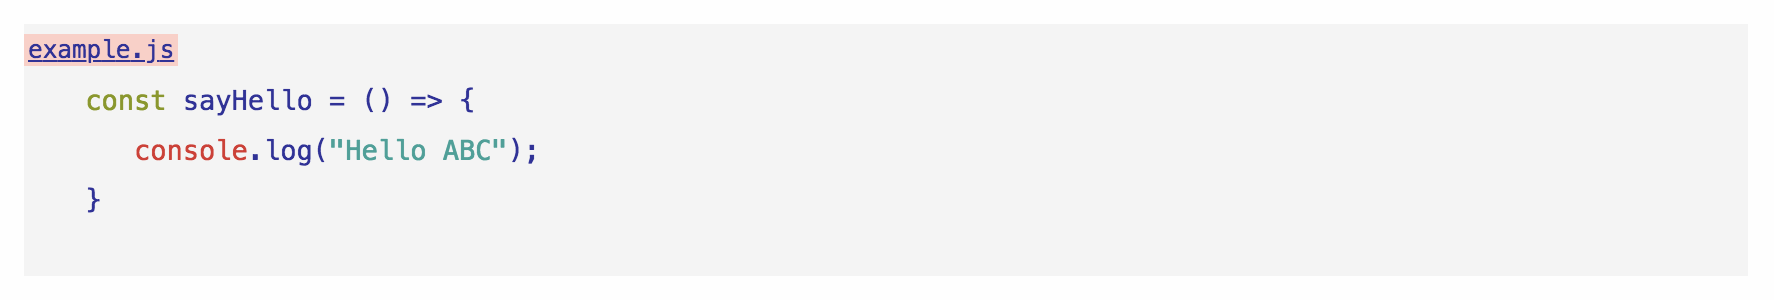
\includegraphics[width=15cm]{images/codeblock.png}
    \caption{コードブロック記法}
    \label{codeblock}
\end{figure}

\begin{figure}[H]
    \centering
    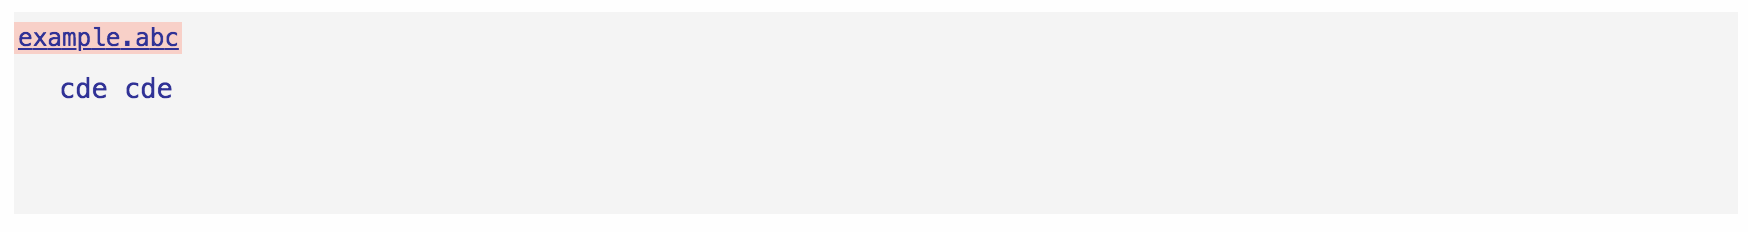
\includegraphics[width=15cm]{images/abcblock.png}
    \caption{ABCとして解釈されるコードブロック}
    \label{abcblock}
\end{figure}

\begin{figure}[H]
    \centering
    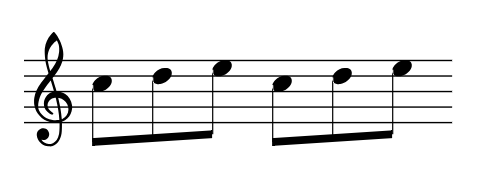
\includegraphics[width=5cm]{images/cdecde.png}
    \caption{生成された楽譜画像}
    \label{cde}
\end{figure}

\section{音符ハイパーリンク機能の実現}
本節では音符ハイパーリンク機能の実現方法を述べる。

abcjsはSVG画像として楽譜を出力しており、一つ一つの音符に対してクリックリスナを設定可能である。
\texttt{Document.location.href}オブジェクト\footnote{\textsf{https://developer.mozilla.org/ja/docs/Web/API/Location}}を利用してページ遷移を実行するコールバック関数を音符のクリックリスナに設定している。
